\chapter{Supplemental figures}
\begin{figure}[thbp]
\centering
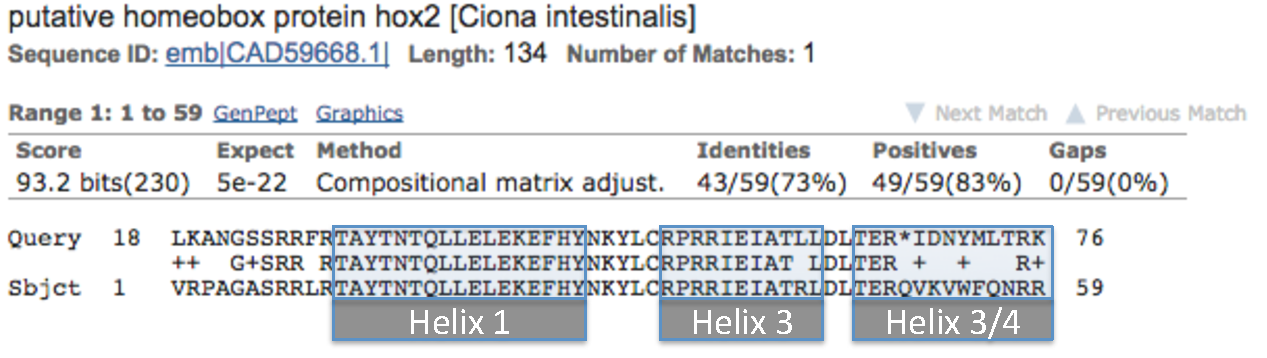
\includegraphics[scale=0.75]{figures/occi_hox2.pdf}
\caption{\textbf{Alignment of \textit{M. occidentalis} \textit{hox2} genes alignment with \textit{Ciona} show  premature stop codon.} \textit{M. occidentalis hox2} gene has a stop codon in the 3' region, inside of the 3/4 helix. \textit{hox2} knockdowns in \textit{Ciona} did not show and phenotypic difference, so the function of \textit{hox2} my not be import in \textit{M. occidentalis} }
\label{fig:occihox2}
\end{figure}

\begin{figure}[tbp]
\centering
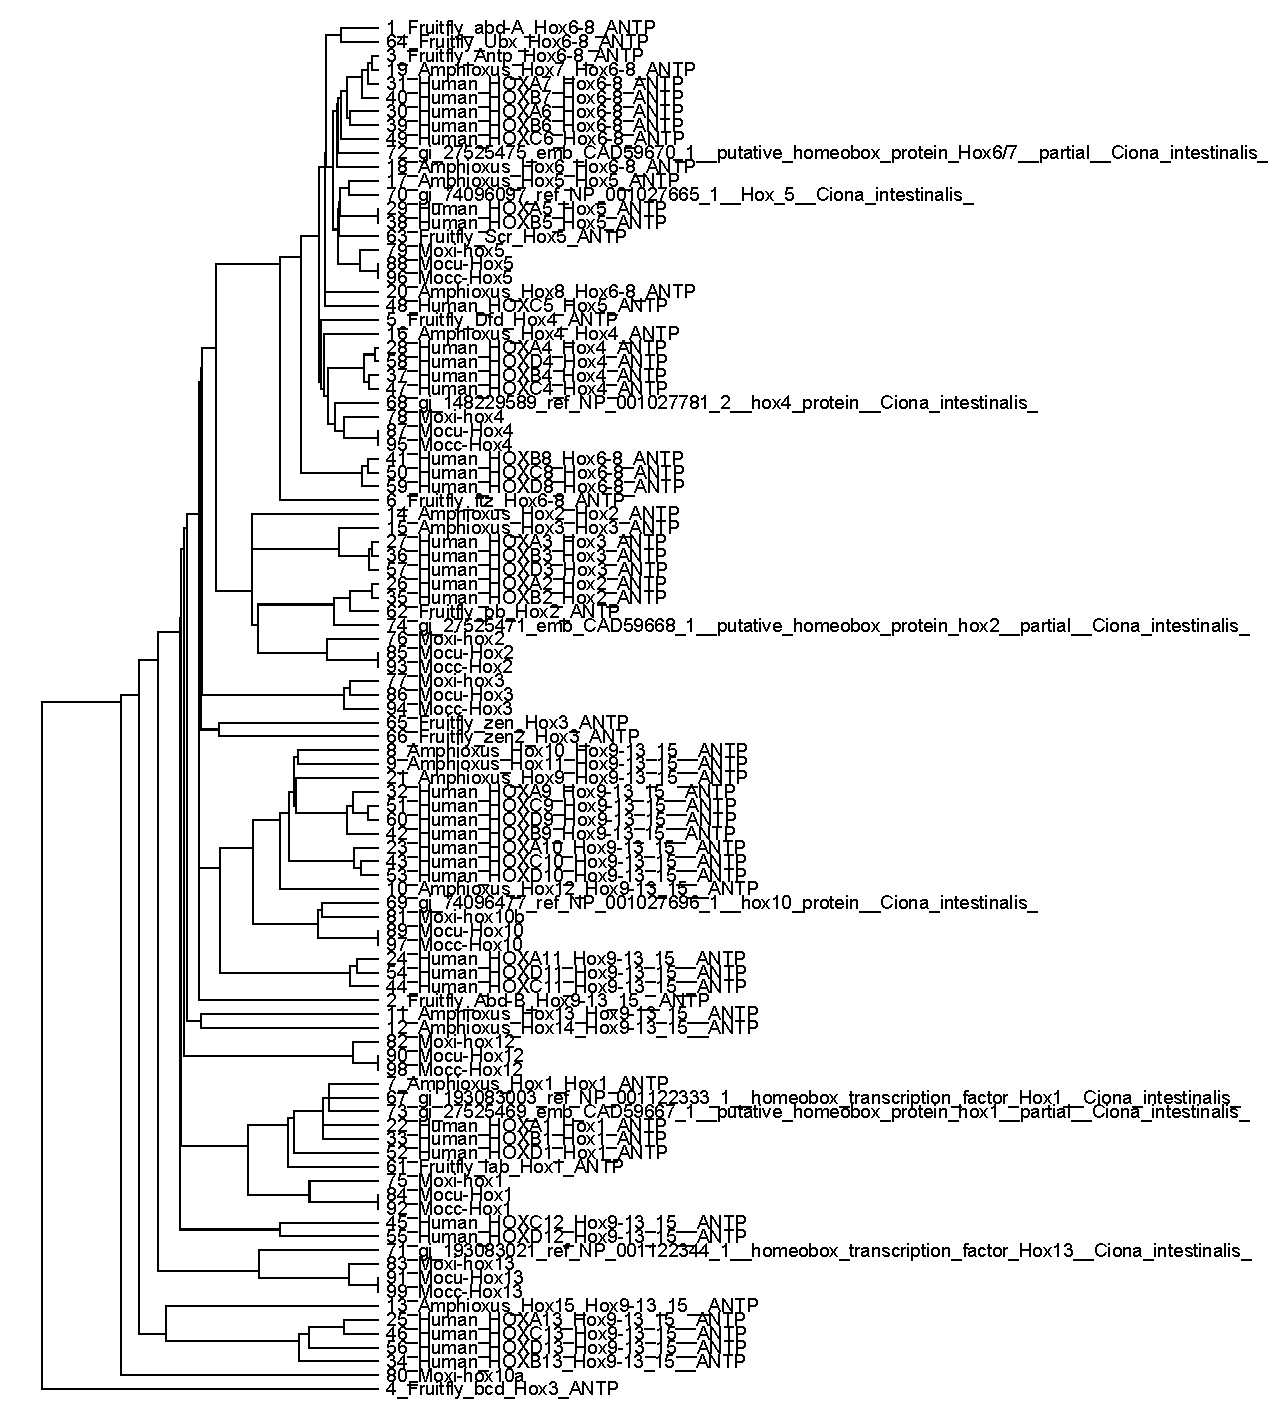
\includegraphics[scale=0.85]{figures/hox_alignment.pdf}
\caption{\textbf{Alignment of \textit{hox} genes.} Alignments of the aa homeobox sequences from all the Molgula species, show that they group with there respective orthologs. All but one of the \textit{M. occidentalis} cluster properly, but \textit{M. occidentalis hox10} full homeobox sequence was not fully assembled, so this is possibly the reason. }
\label{fig:hox-alignments}
\end{figure}

\begin{figure}[tbp]
\centering
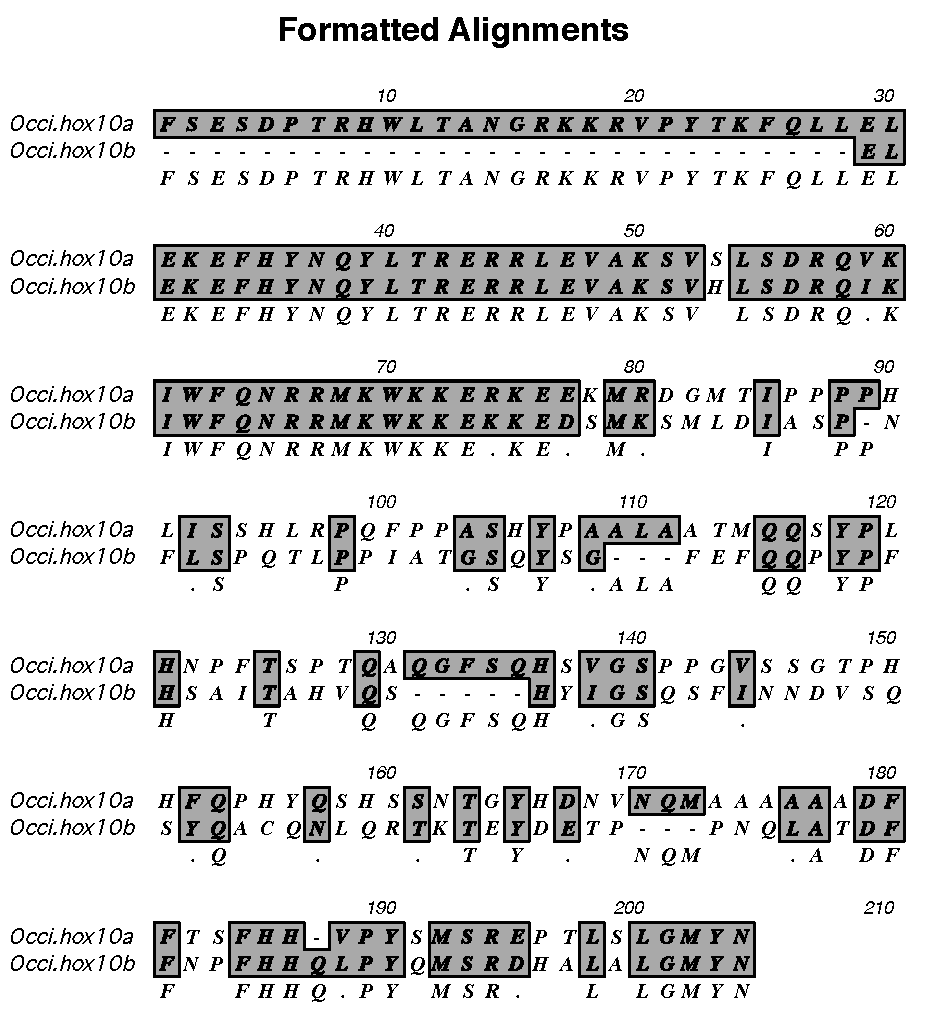
\includegraphics[scale=0.95]{figures/Occi_hox10.pdf}
\caption{\textbf{Alignment of \textit{M. occidentalis} duplicate \textit{hox10} genes} Two copies of \textit{hox10} were found in \textit{M. occidentalis} \mytilde12 kb apart on the same contig.}
\label{fig:occihox10}
\end{figure}

\begin{figure}[tbp]
\centering
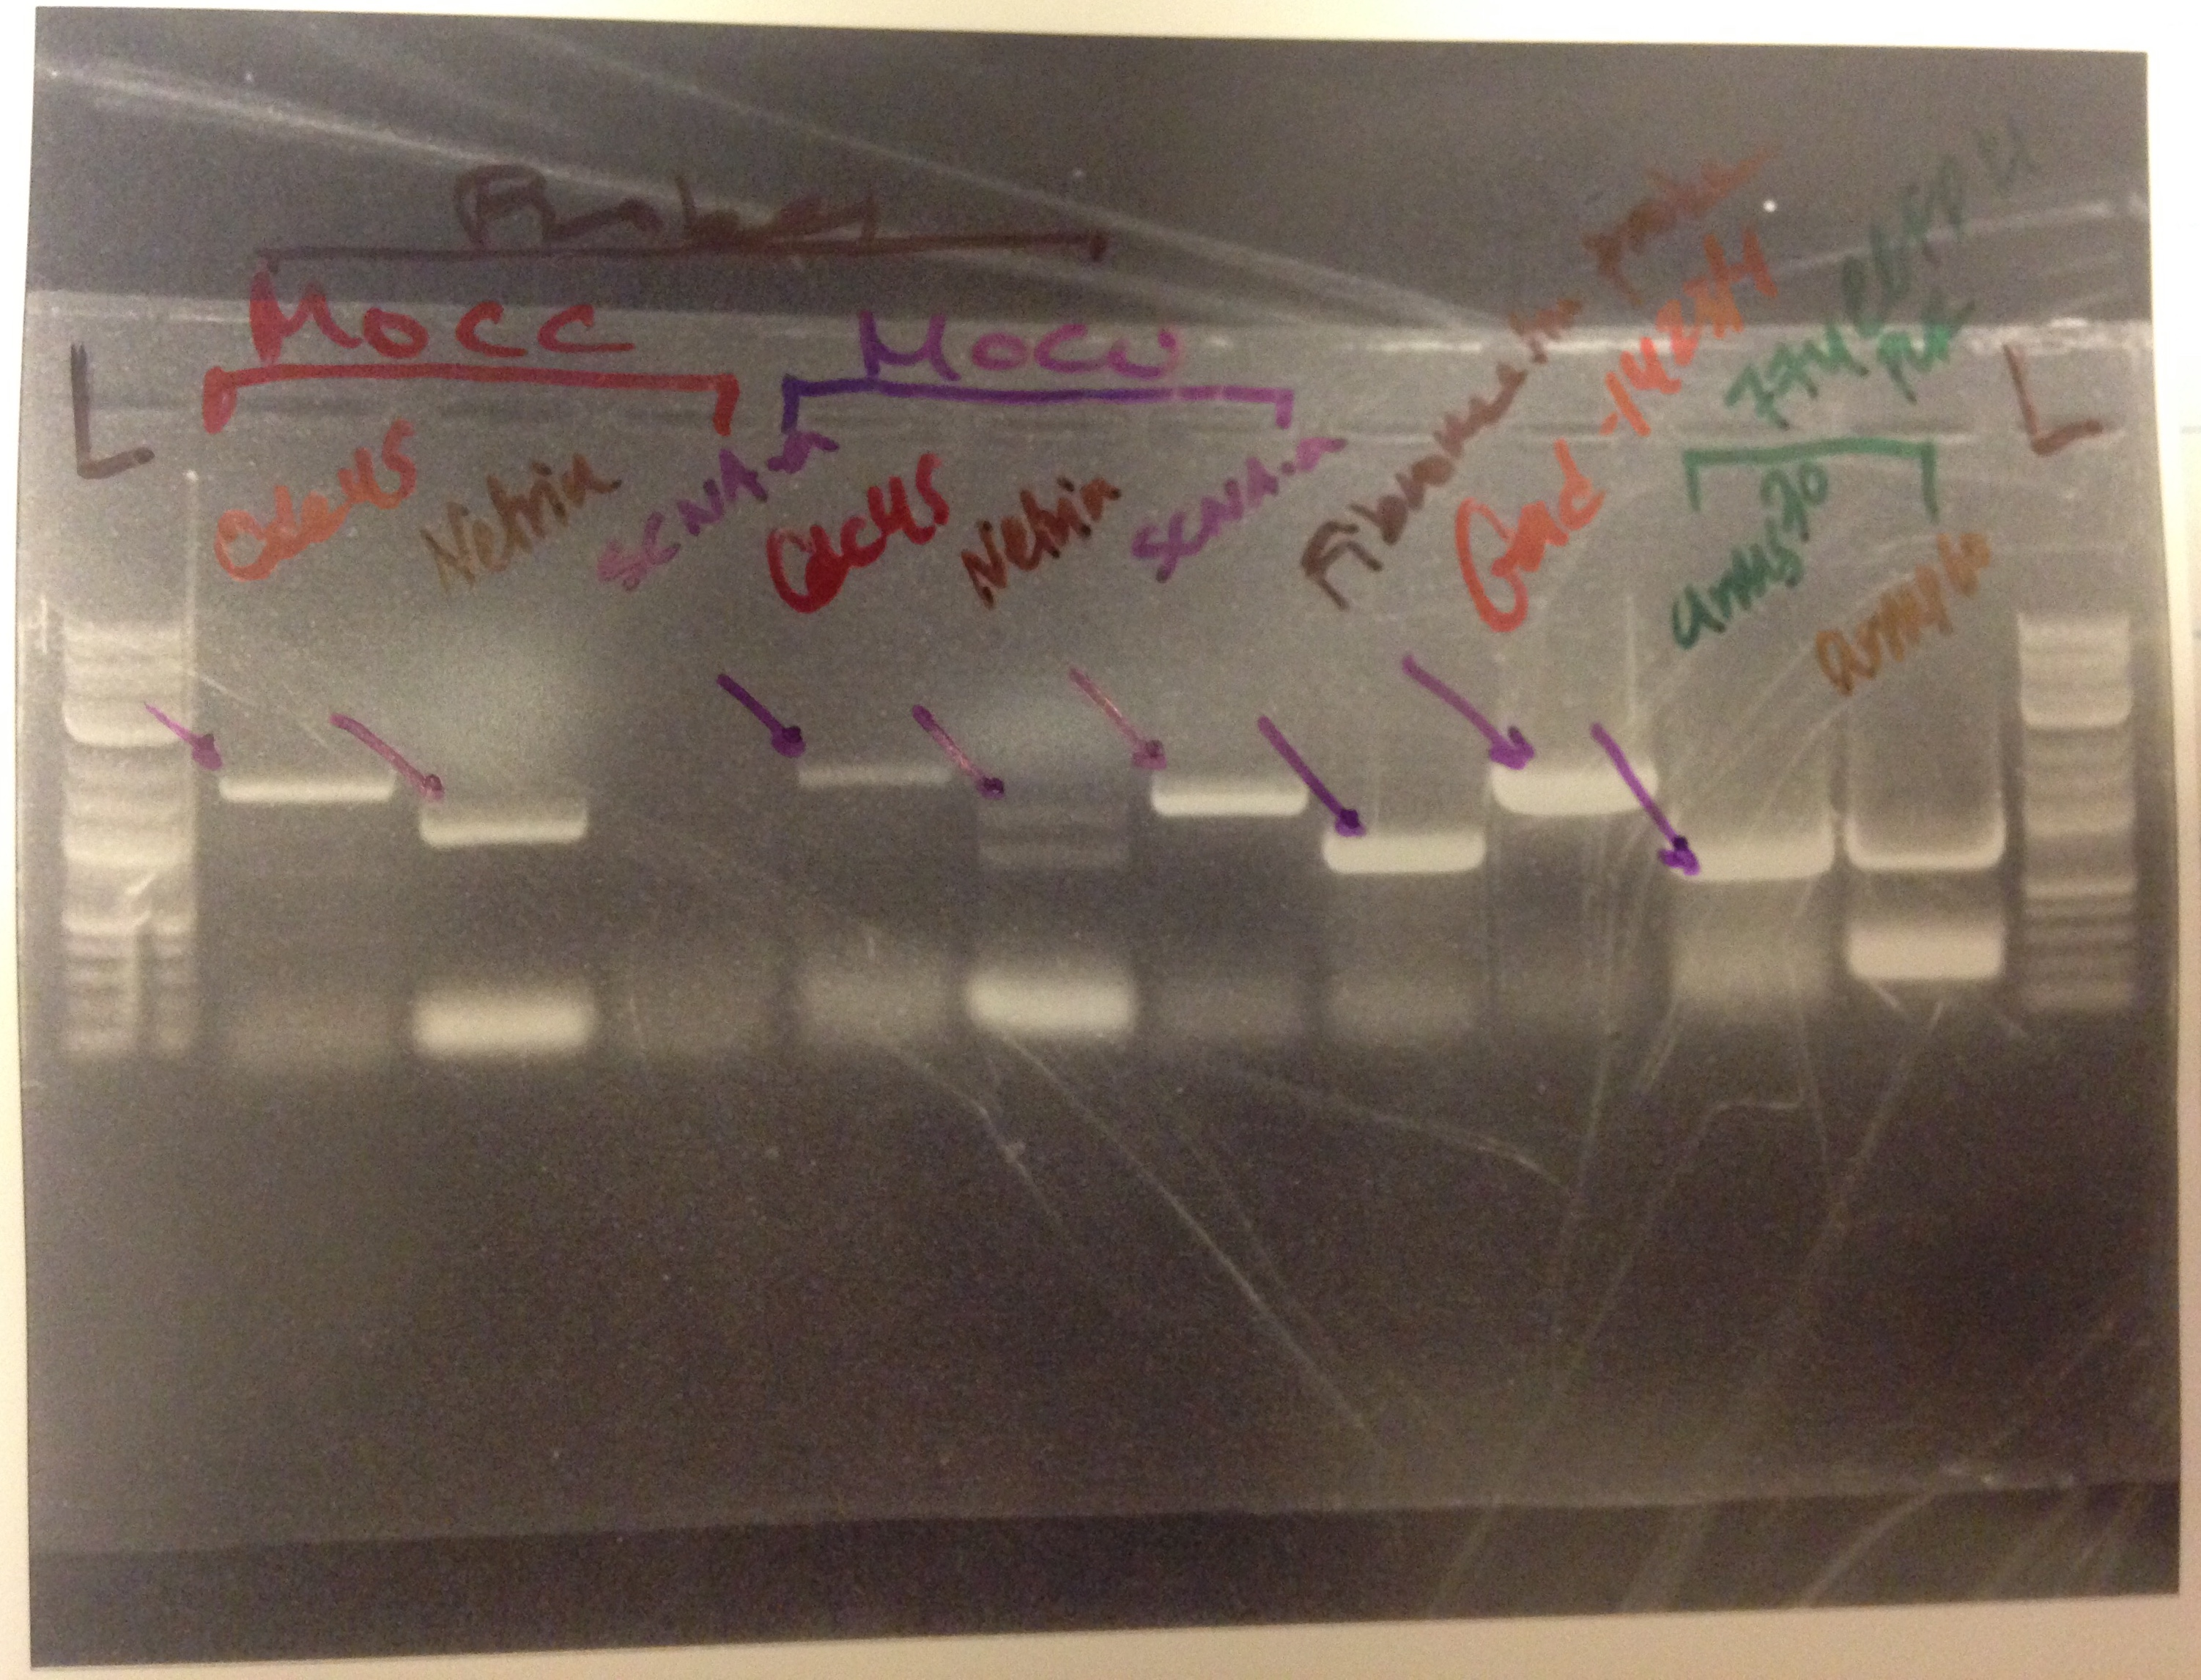
\includegraphics[scale=0.10]{figures/gel.jpg}
\caption{\textbf{Gel of cdc45, netrin and controls} \textit{Netrin} was not found in \textit{M. occulta's} transcriptome but was recovered via PCR. However, this library has a wider ranger of developmental stages, so it is still possible \textit{netrin} is not expressed at the right stage for tail development.}
\label{fig:gel}
\end{figure}

\begin{figure}[tbp]
\centering
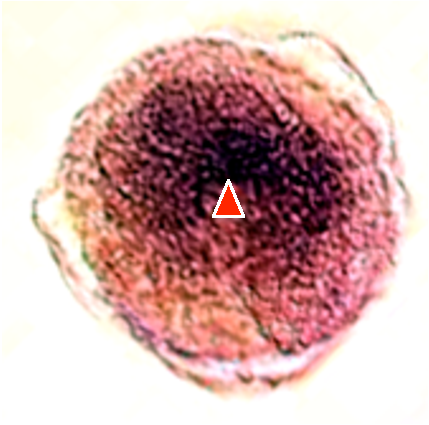
\includegraphics[scale=0.55]{figures/prickle.pdf}
\caption{\textbf{Whole Mount In Situ Hybridization of \textit{prickle} in \textit{M. occulta}} The PCP gene \textit{pk} was shown to be expressed in the notochord in a similar pattern to \textit{C. intestinalis} }
\label{fig:prickle}
\end{figure}